\documentclass[11pt,a4paper]{article}

\usepackage[margin=0.9in]{geometry}
\usepackage{graphicx}
\usepackage{pdfpages}
\usepackage{booktabs}
\usepackage{float}
\usepackage{natbib}
\usepackage{newtxtext,newtxmath}
\usepackage[hidelinks]{hyperref}

\graphicspath{{./}}
\emergencystretch=2em

\title{Kramer annulus Stokes benchmark}
\author{}
\date{}

\begin{document}

\maketitle
\vspace{-2.0em}

\section{Introduction}

The Kramer annulus benchmark verifies incompressible Stokes flow in a two-dimensional cylindrical shell using the analytical solutions of \citet{kramer2021}. This benchmark is relevant to mantle-convection modelling because it tests curved boundaries, free-slip and zero-slip velocity conditions, pressure normalisation, and both smooth and interface-localised buoyancy forcing. The annulus configuration is also a useful intermediate verification problem: it contains the same geometric and boundary-condition issues as spherical-shell calculations, but with lower dimensional cost and simpler visualisation.

\section{Benchmark setup}

The model solves
\[
  -\nabla\cdot\boldsymbol{\sigma}=\rho\mathbf{g},
  \qquad
  \nabla\cdot\mathbf{u}=0,
\]
with constant viscosity in an annulus with radii \(R_-=1.22\) and \(R_+=2.22\). Delta-function cases use an internal circular interface at \(R_{\mathrm{int}}=2.0\). Smooth forcing is proportional to \((r/R_+)^k\cos(n\theta)\), while delta-function forcing is proportional to \(\delta(r-R_{\mathrm{int}})\cos(n\theta)\). The UW3 calculations use \(P_2\)--\(P_1\) Taylor--Hood elements, with quadratic velocity and continuous linear pressure. Mesh sizes are \(h=1/8,\ldots,1/256\). Cases 1 and 2 use free-slip boundaries; Cases 3 and 4 use zero-slip boundaries.

\begin{table}[H]
\centering
\caption{Kramer annulus benchmark cases used in the UW3 verification runs.}
\label{tab:annulus_cases}
\begin{tabular}{cllll}
\toprule
Case & Forcing & Boundary condition & Parameters & Resolutions \\
\midrule
1 & delta-function & free-slip & \(n=2,8,32\) & \(1/8\)--\(1/256\) \\
2 & smooth & free-slip & \(n=2,8,32;\ k=2,8\) & \(1/8\)--\(1/256\) \\
3 & delta-function & zero-slip & \(n=2,8,32\) & \(1/8\)--\(1/256\) \\
4 & smooth & zero-slip & \(n=2,8,32;\ k=2,8\) & \(1/8\)--\(1/256\) \\
\bottomrule
\end{tabular}
\end{table}

\section{Analytical density fields}

\begin{figure}[H]
    \centering
    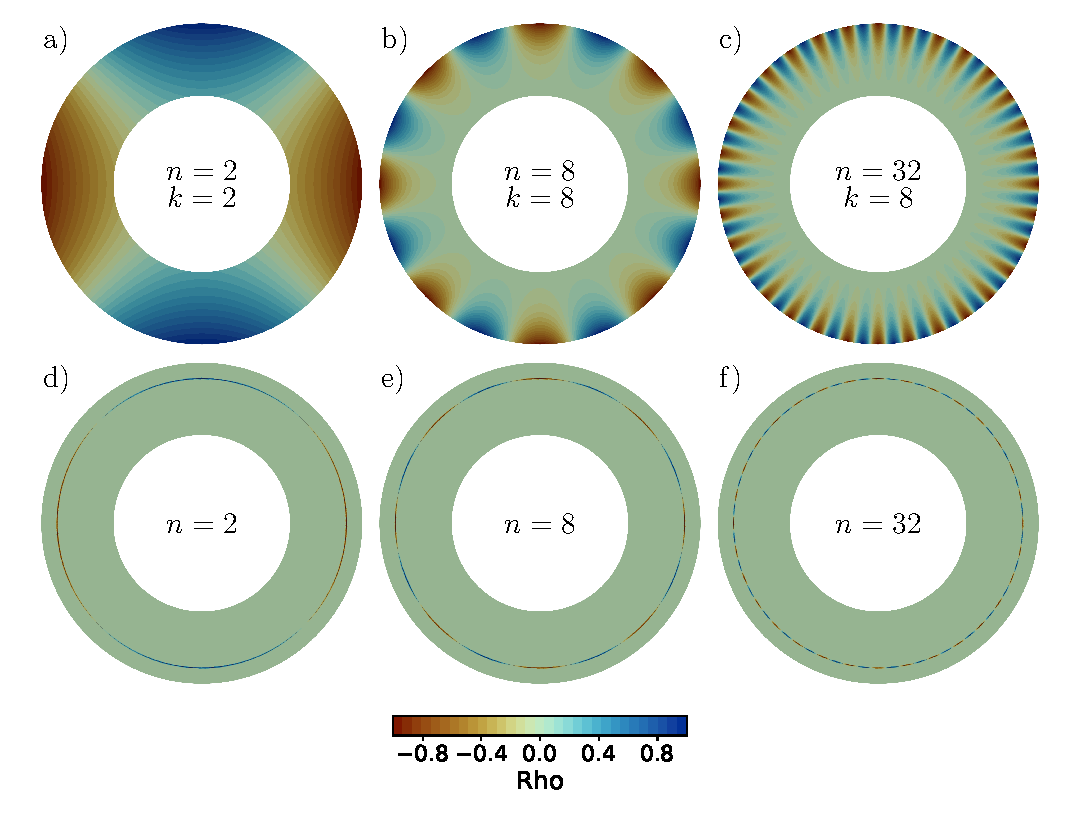
\includegraphics[width=0.98\linewidth]{figure_1_kramer_annulus_rho_ana.pdf}
    \caption{Analytical density perturbations for the annulus Kramer benchmark. The upper row shows smooth forcing and the lower row shows delta-function forcing. Columns correspond to increasing azimuthal complexity.}
    \label{fig:annulus_density}
\end{figure}

Figure~\ref{fig:annulus_density} shows the imposed density fields used for the convergence tests. Increasing \(n\) increases the azimuthal wavenumber and therefore the angular complexity of the forcing. For smooth forcing, \(k\) controls radial variation and concentrates structure differently across the shell. For delta-function forcing, the density is localised on the internal interface, reducing solution regularity relative to the smooth cases.

\section{Velocity and pressure convergence}

\begin{figure}[H]
    \centering
    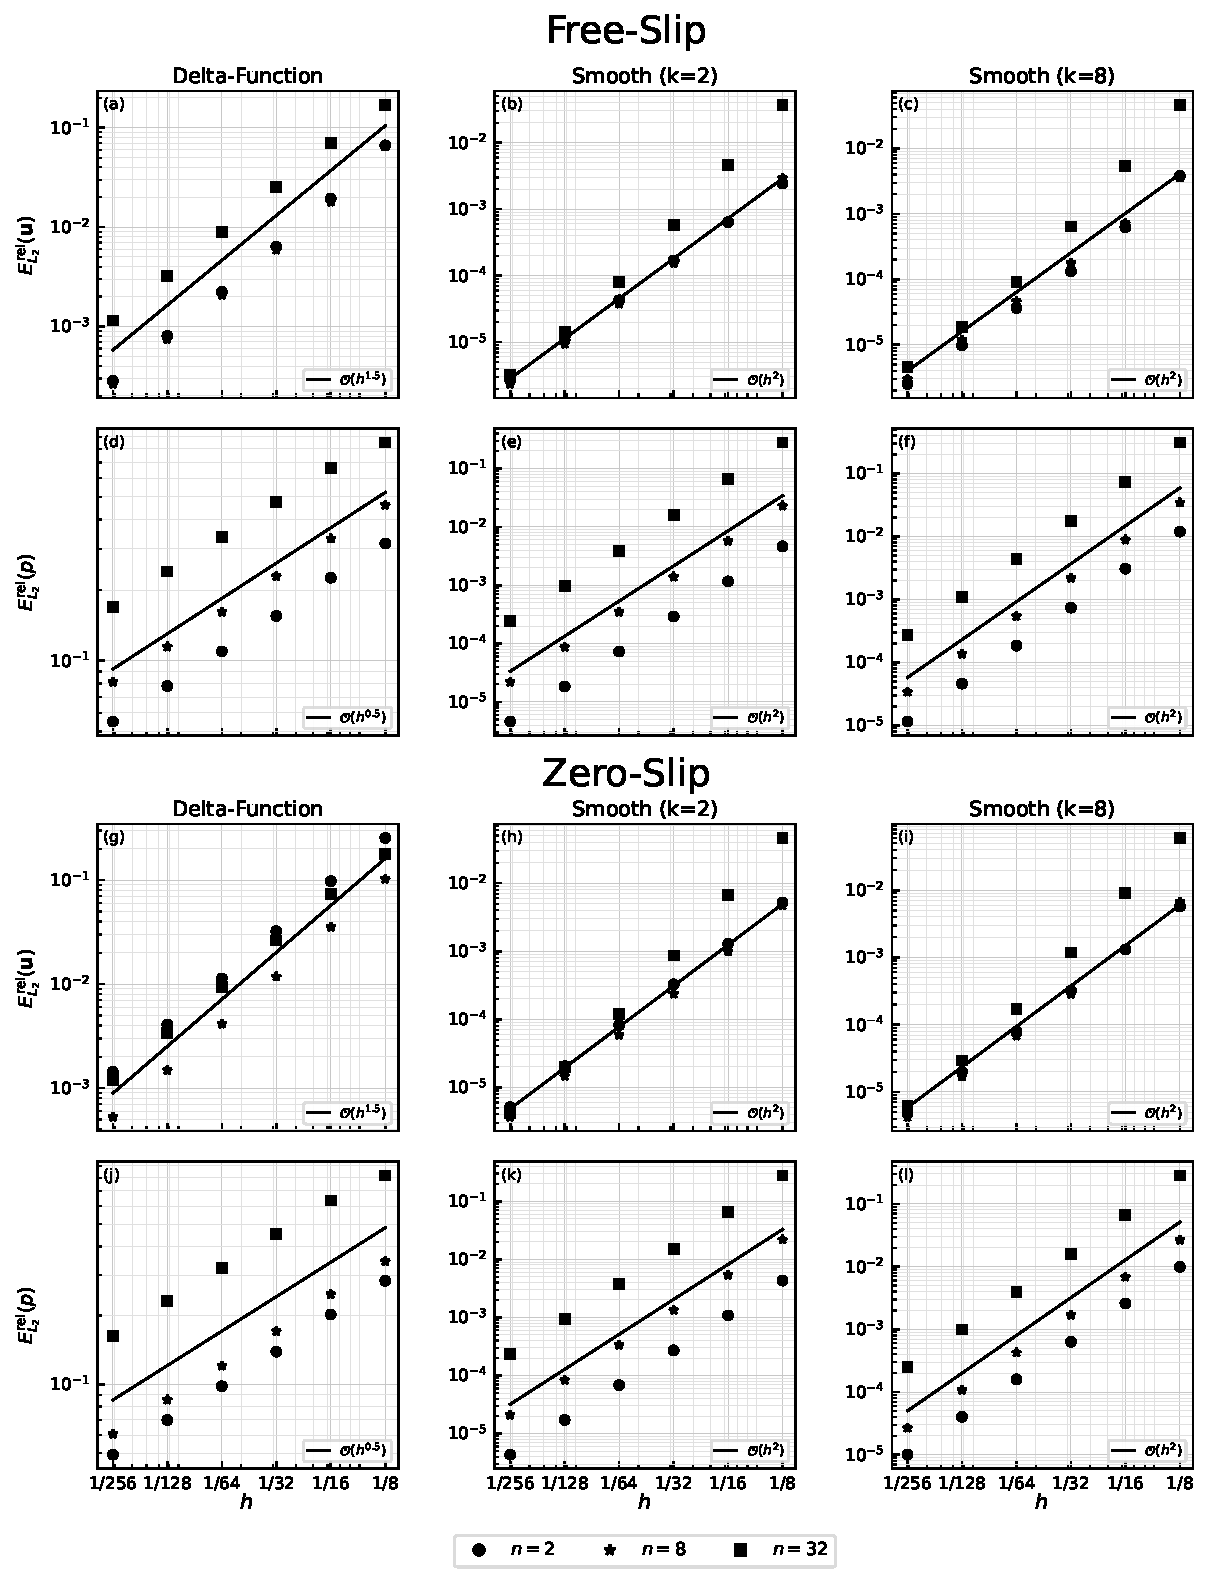
\includegraphics[width=0.98\linewidth]{figure_3_kramer_annulus_convergence.pdf}
    \caption{Velocity and pressure convergence for the four annulus Kramer cases. Columns show delta-function forcing and smooth forcing with \(k=2\) and \(k=8\). The upper block uses free-slip boundaries and the lower block uses zero-slip boundaries.}
    \label{fig:annulus_convergence}
\end{figure}

Velocity and pressure errors are reported as relative volume \(L_2\) norms. For smooth Stokes solutions, the \(P_2\)--\(P_1\) pair can exhibit third-order velocity convergence and second-order pressure convergence in the \(L_2\) norm, provided the curved geometry and boundary conditions are represented accurately \citep{girault1986,boffi2013}. The UW3 annulus results show robust convergence for all cases. For smooth forcing, pressure converges close to \(O(h^2)\) for both free-slip and zero-slip boundaries. Smooth velocity convergence is approximately second order for \(n=2\) and \(n=8\), while the high-wavenumber \(n=32\) cases show higher, pre-asymptotic rates that approach the expected smooth-solution trend over refinement.

The delta-function cases show the reduced rates expected for interface-localised forcing. Velocity convergence approaches \(O(h^{1.5})\) and pressure convergence approaches \(O(h^{0.5})\) for both free-slip and zero-slip boundaries. This is consistent with the Fluidity results of \citet{kramer2021} and reflects reduced regularity introduced by the internal forcing interface rather than a solver failure. The continuous pressure discretisation is especially sensitive to this reduced regularity, explaining the systematically slower pressure convergence in Cases 1 and 3.

\section{Discussion}

The convergence behaviour separates cleanly by forcing type. Smooth cases retain second-order pressure convergence and generally second-order or better velocity convergence. Delta-function cases show suboptimal but systematic convergence, with rates matching the reduced regularity expected from the Green's-function solution. Increasing \(n\) increases angular complexity and raises error constants, especially in the pressure norm. This is visible in both the plotted errors and the tabulated values.

The free-slip and zero-slip cases follow the same qualitative trends, indicating that the boundary-condition implementations are consistent for the annulus benchmark. Differences in constants between the two boundary conditions are expected because the admissible velocity space and boundary constraints differ. The smooth velocity results are not uniformly third order over all \(n\), despite the \(P_2\) velocity approximation. This suggests that geometry representation, boundary enforcement, or resolution relative to high-wavenumber forcing controls the observed error before the full asymptotic interpolation rate is reached. The additional \(O(h^2)\) and \(O(h^3)\) reference lines in Fig.~\ref{fig:annulus_convergence} make this transition visible.

\section{Tabulated errors}

The numerical values and pairwise convergence rates are provided in the following pages. Each table groups the three azimuthal wavenumbers and reports \(h\), velocity error, velocity rate, pressure error, and pressure rate.

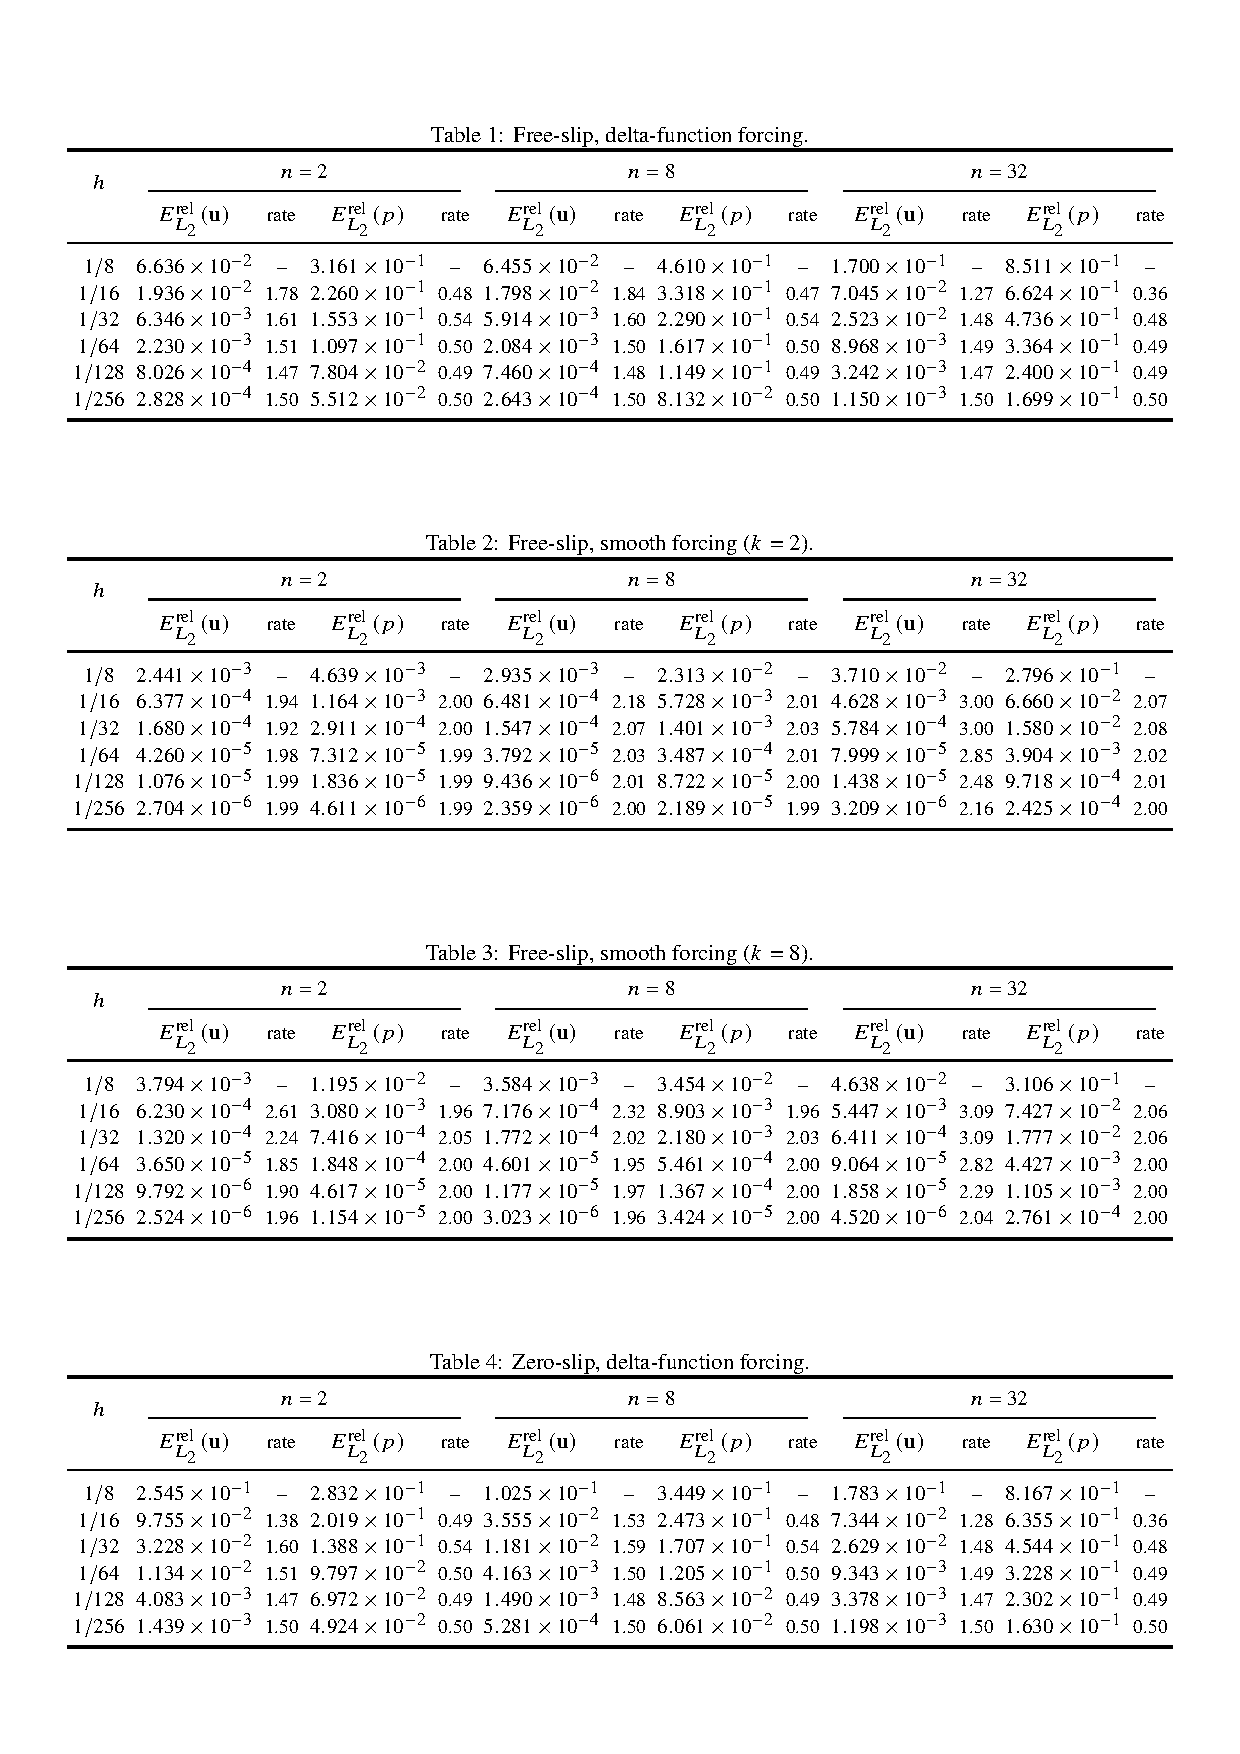
\includepdf[pages=-,fitpaper=true,pagecommand={\thispagestyle{plain}}]{table_figure_3_kramer_annulus_convergence.pdf}

\section{Summary}

The UW3 annulus benchmark reproduces the principal results of \citet{kramer2021}. Smooth pressure converges at the expected second-order rate, and smooth velocity converges systematically with rates close to second order or higher depending on wavenumber and resolution. Delta-function forcing produces the expected reduced convergence, approximately \(O(h^{1.5})\) in velocity and \(O(h^{0.5})\) in pressure. These results verify the UW3 annulus Stokes implementation for curved-shell geometry, free-slip and zero-slip boundaries, and both volumetric and interface-localised buoyancy forcing.

\bibliographystyle{plainnat}
\bibliography{kramer_annulus_benchmark_report_refs}

\end{document}
